\chapter{Android 6 – Services, Broadcast Receiver, App- Design \& Publikation}

\section{Services}

Mit einem Service kann man dem System mitteilen, dass eine bestimmte Arbeit im Hintergrund erledigt werden soll. Zudem lassen sich gewisse Funktionalitäten exportieren und so anderen Applikationen zur Verfügung gestellt. Ein Service läuft standardmässig nicht in einem separaten Thread (läuft im main-Thread) und auch nicht in einem eigenen Prozess (nur wenn so definiert). Deshalb sollte der Service einen Thread starten, um lang andauernde Operationen zu erledigen. Ein Service sollte benutzt werden wenn die Hintergrund-Aktivität weiterlaufen soll, auch wenn die Activity nicht mehr sichtbar ist (z.B. Musik läuft weiter). Soll die Aktivität beendet werden, wenn die Activity nicht mehr sichtbar ist sollte ein Worker-Thread verwendet werden (z.B. Animation soll stoppen). Es gibt gebundene Services und ungebundene Services, welche nachfolgend beschrieben werden.

\subsection{Ungebundene Services}

Ein ungebundener Service wird mit der Methode \texttt{startService(...)} gestartet und durchläuft folgenden Lebenszyklus:
\begin{description}
	\item[onCreate:] Bei Erzeugung
	\item[onStartCommand:] Auftragsbehandlung
	\item[onDestroy:] Bei Beendung (durch Service selbst, durch Applikation oder durch System)
\end{description}
Der Service bleibt so lange im RUNNING Zustand bis er explizit beendet wird. Abbildung \ref{fig:service} zeigt wie ein Service verwendet wird. Zudem muss man den Service noch mit Manifest deklarieren. 

\begin{figure}
	\centering
	\begin{subfigure}[b]{0.48\textwidth}
		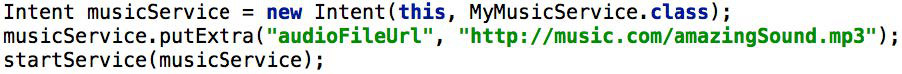
\includegraphics[width=\textwidth]{fig/service-starten}
		\caption{Service starten}
	\end{subfigure}
	~
	\begin{subfigure}[b]{0.48\textwidth}
		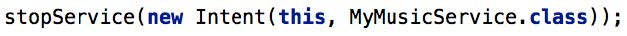
\includegraphics[width=\textwidth]{fig/service-stoppen}
		\caption{Service stoppen}
	\end{subfigure}
	~
	\begin{subfigure}[b]{0.48\textwidth}
		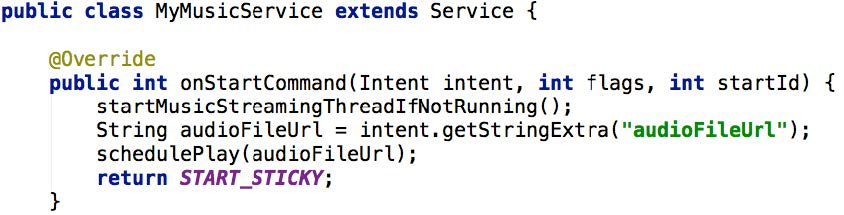
\includegraphics[width=\textwidth]{fig/service-implementierung}
		\caption{Service Implementierung}
	\end{subfigure}
	\caption{Service}
	\label{fig:service}
\end{figure}

Wenn ein Service von der Klasse \texttt{Service} ableitet, muss die Methode \texttt{onStartCommand()} implementiert werden. Es können mehrere Aufrufe von \texttt{onStartCommand()} erfolgen, auch wenn der Service noch einen Auftrag abhandelt. Dadurch wird eine parallele Abhandlung möglich jedoch muss auch eine komplizierte Kommunikation zwischen den Threads erfolgen.
Wenn ein Service von der Klasse \texttt{IntentService} ableitet, muss die Methode \texttt{onHandleIntent()} implementiert werden. Wird der Service aufgerufen erfolgt der neue Auftrag erst, wenn der vorige Job abgeschlossen ist. Demzufolge läuft die Methode \texttt{onHandleIntent()} automatisch in einem Worker-Thread.
Mit dem Rückgabewert von der Methode \texttt{onStartCommand()} kann das Verhalten des Service definiert werden, wenn die Applikation zerstört und später wiederhergestellt wird (nicht wichtig für gebundene Services weil existieren so lange wie Binding). Es gibt folgende Rückgabewerte:
\begin{description}
	\item[START\_STICKY:] Service soll nach Wiederherstellung automatisch gestartet werden -- \\ \texttt{onStartCommand()} wird erneut aufgerufen, aber ohne Intent
	\item[START\_NOT\_STICKY:] Service wird nicht automatisch neu gestartet nach Wiederherstellung
	\item[START\_REDELIVER\_INTENT:] Wie START\_STICKY, aber der ursprüngliche Intent wird noch einmal ausgeliefert, damit parametrisierte Reinitialisierung möglich
\end{description}

\subsection{Gebundene Services}

Ein gebundener Service wird mit der Methode \texttt{bindService(...)} gestartet und durchläuft folgenden Lebenszyklus:
\begin{description}
	\item[onCreate:] Bei Erzeugung
	\item[onBind:] Wenn Komponente Verbindung herstellt
	\item[onUnbind:] Wenn Komponente Verbindung beendet
	\item[onDestroy:] Bei Beendung (durch Service selbst, durch Applikation oder durch System)
\end{description}
Der Service bleibt so lange im RUNNING Zustand wie das Binding existiert. Der Client kommuniziert mit der Klasse \texttt{ServiceConnection} mit dem Service. Mit der Methode \texttt{unbindService(connection)} wird die Bindung aufgelöst. Bei einem gebundenen Service sind folgende Klassen involviert:
\begin{description}
	\item[Service Interface:] Definiert API des Services
	\item[Binder:] Implementiert Service Interface, wird dem Client bei erfolgreicher Verbindung übergeben
	\item[Service Connection:] Definiert Callbacks für erfolgreiche Verbindung oder verlorene Verbindung, erhält Binder-Objekt bei Erfolg
	\item[Service:] Implementiert \texttt{onBind(intent)} und gibt Binder-Objekt zurück
	\item[Client:] Ruft \texttt{bindService(intent, connection, flag)} resp. \texttt{unbindService(connnection)} auf
\end{description}
Abbildung \ref{fig:gebundener-service} zeigt den Ablauf eines Service Bindings.

\begin{figure}
\centering
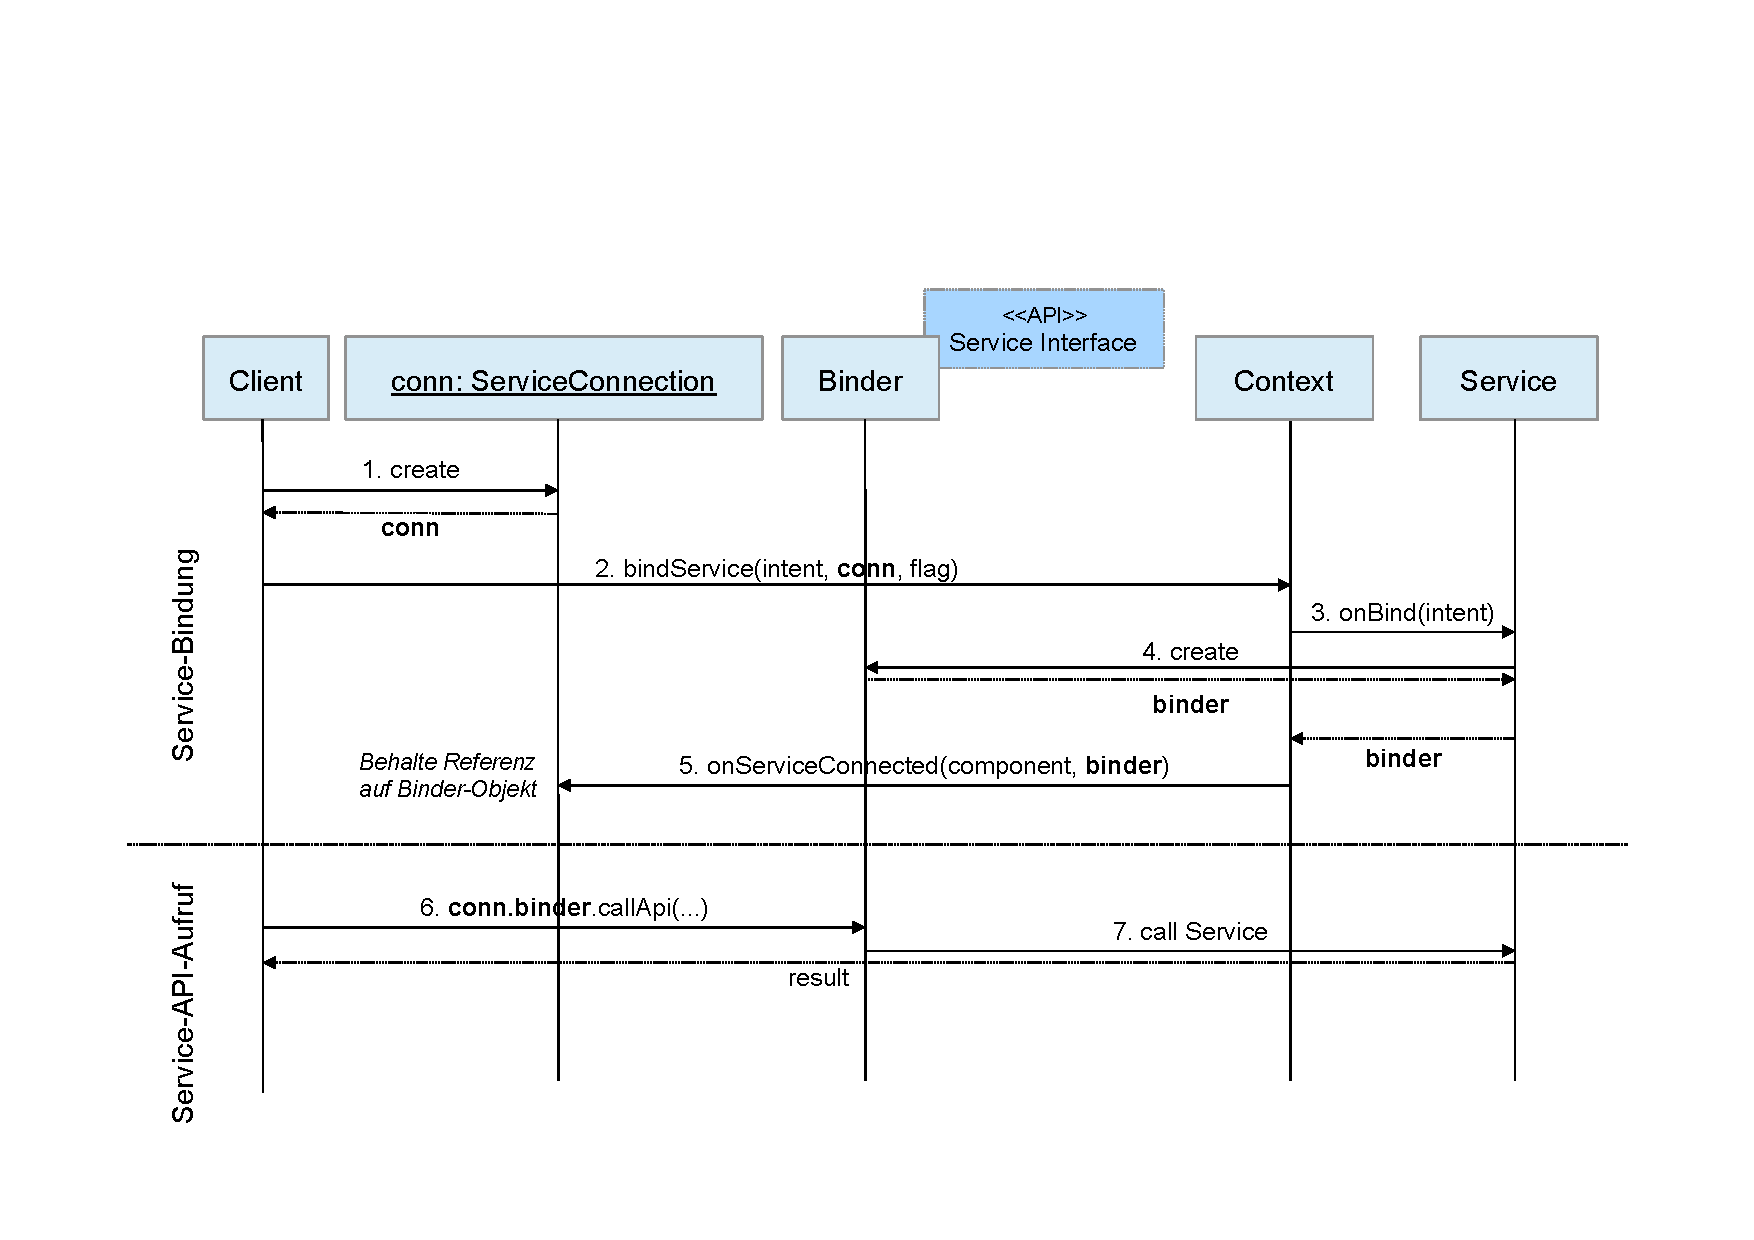
\includegraphics[width=0.7\linewidth]{fig/gebundener-service}
\caption{Seqeuenzdiagramm gebundener Service}
\label{fig:gebundener-service}
\end{figure}

\section{Broadcast Receiver}

Broadcast sind Systemnachrichten welche vom Android-System verschickt werden (z.B. \texttt{BOOT\_COMPLETED}, \texttt{BATTERY\_CHANGED}). Alle Apps können Broadcasts mit via Intent verschicken (\texttt{sendBroadcast(intent)}). Broadcast-Intents werden an registrierte \texttt{BroadcastReceiver} (im gesamten System!) weitergeleitet. Ein \texttt{BroadcastReceiver} kann entweder dynamisch registriert oder im Manifest definiert werden. Ein \texttt{BroadcastReceiver} ist nur solange aktiv, wei die Bearbeitung der empfangenen Nachricht braucht (wird danach gelöscht und neu erzeugt \emph{on demand}). Deshalb sollte man im \texttt{BroadcastReceiver} keine AsyncTasks, kein Service und keine Dialoge zeigen. Abbildung \ref{fig:broadcast-receiver} zeigt wie \texttt{BroadcastReceiver} erzeugt werden können.

\begin{figure}
	\centering
	\begin{subfigure}[b]{0.48\textwidth}
		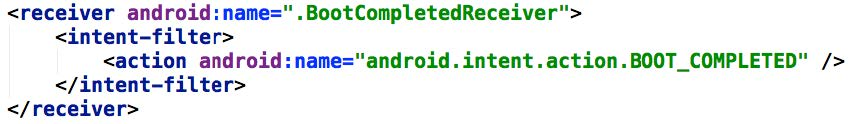
\includegraphics[width=\textwidth]{fig/broadcast-receiver-manifest}
		\caption{Deklarieren im Manifest}
	\end{subfigure}
	~
	\begin{subfigure}[b]{0.48\textwidth}
		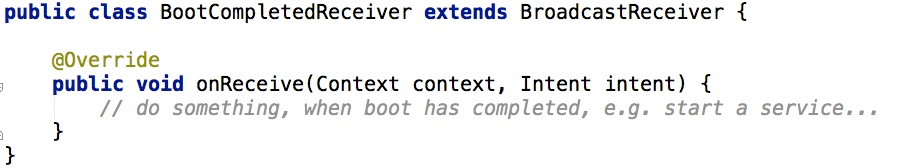
\includegraphics[width=\textwidth]{fig/broadcast-receiver-manifest-klasse}
		\caption{Dedizierte Klasse}
	\end{subfigure}
	~
	\begin{subfigure}[b]{0.48\textwidth}
		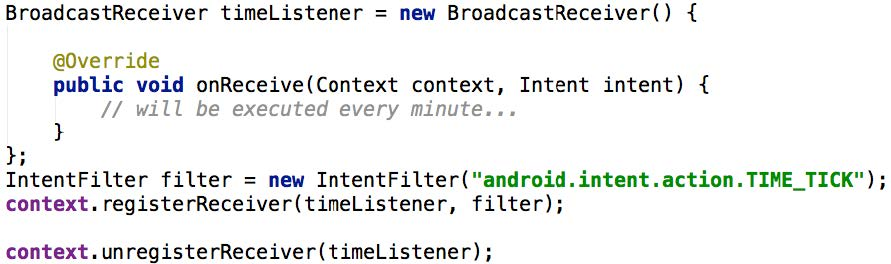
\includegraphics[width=\textwidth]{fig/broadcast-receiver-dynamisch}
		\caption{Dynamisch registrieren}
	\end{subfigure}
	\caption{Broadcast Receiver erzeugen}
	\label{fig:broadcast-receiver}
\end{figure}
Es können auch eigene Broadcast-Actions definiert werden.

\section{Hinweise zum App-Design \& Usability}

Android-Doku erläutert, wie Apps designed sein sollen, wie Widgets und Styles aussehen, wie einsetzen usw. Das Design ist ein iterativer Prozess der zusammen mit dem Kunden durchgeführt werden sollte. Prototypen helfen da sehr. Man kann ein Prototyp auf Papier oder mit einem SW-Tool erstellen und sollte mit diesem dann die App durchspielen. 

\section{Publikation von Apps}

Um Apps zu veröffentlichen braucht man einen Google Account (Gratis), ein Google Play Publisher Account (\$25, einmalig) und für kostenpflichtige Apps ein Google Wallet Merchant Account (30\% für Google 70\% für Entwickler). Nachfolgend wird grob das Vorgehen der Publikation beschrieben:
\begin{enumerate}
	\item Code Cleanup, Release vorbereiten (Versionierung, Internationalisierung, Logging entfernen, etc.)
	\item Release erstellen und signieren
	\item Werbematerial vorbereiten (Screenshots, Hi-Res Icon, Feature, Promo, Video, Website)
	\item Distributionseinstellungen setzen (Content Rating, Verfügbarkeit, Grösse, Bezahlung: Gratis, Kostenpflichtig, In-App?)
	\item Release hochladen und veröffentlichen
\end{enumerate}
Apps werden im APK (Android Application Package) verteilt. Der ganze Programmcode (.dex) und alle Ressourcen (Manifest, Zertifikat usw.) werden in ein zip-File gepackt und mit der Dateiendung .apk gespeichert.
Mit ProGuard kann den Source Code optimieren und obfuskieren, damit das Reverse Engineering schwieriger wird. Allerdings bietet diese Technik nur einen geringen Schutz.
Apps müssen für den Play Store signiert werden (self-siging erlaubt). Updates sollten mit gleichem Zertifikat signiert werden, sonst muss der Package Name geändert werden!
Apps können auch in alternativen Stores (AppBrain, Amazon Appstore) oder einfach als .apk-Datei versendet werden. Apps können zudem mit JUnit 3 getestet werden. Es sind auch automatisierte UI-Tests möglich.
